\documentclass[unicode,12pt,aspectratio=169]{beamer}

\usepackage{luatexja}% 日本語したい
\usepackage[haranoaji,no-math,deluxe,expert,nfssonly,match,scale=1.0]{luatexja-preset}
\renewcommand{\kanjifamilydefault}{\gtdefault}% 既定をゴシック体に

\usepackage{amssymb,amsmath,ascmac}

\usepackage{multirow}
\usepackage{lltjext}

\usepackage{siunitx}
\usepackage{physics}
\AtBeginDocument{\RenewCommandCopy\qty\SI}
\ExplSyntaxOn
\msg_redirect_name:nnn { siunitx } { physics-pkg } { none }
\ExplSyntaxOff

\usepackage{animate}
\usepackage{svg}
\usepackage{tikz}
\usepackage{xparse}
%%%%%%%%%%%%%%%%%%%%%%%
\graphicspath{{../fig/}}
%%%%%%%%%%%%%%%%%%%%%%%%%%%
\usetikzlibrary{shapes,arrows}
\usetikzlibrary{positioning}
\usetikzlibrary{angles,quotes}
\usetikzlibrary{math, calc}
\usetikzlibrary{decorations.markings,decorations.pathmorphing}
%% define fancy arrow. \tikzfancyarrow[<option>]{<text>}. ex: \tikzfancyarrow[fill=red!5]{hoge}
\tikzset{arrowstyle/.style n args={2}{inner ysep=0.1ex, inner xsep=0.5em, minimum height=2em, draw=#2, fill=black!20, font=\sffamily\bfseries, single arrow, single arrow head extend=0.4em, #1,}}
\NewDocumentCommand{\tikzfancyarrow}{O{fill=black!20} O{none}  m}{
\tikz[baseline=-0.5ex]\node [arrowstyle={#1}{#2}] {#3 \mathstrut};}

%目次スライド
% \AtBeginSection[]{
%   \frame{\tableofcontents[currentsection]}
% }
%アペンディックスのページ番号除去
\newcommand{\backupbegin}{
\newcounter{framenumberappendix}
\setcounter{framenumberappendix}{\value{framenumber}}
}
\newcommand{\backupend}{
\addtocounter{framenumberappendix}{-\value{framenumber}}
\addtocounter{framenumber}{\value{framenumberappendix}} 
}

%%%%%%%%%%%  theme  %%%%%%%%%%%
% \usetheme{Copenhagen}
\usetheme{metropolis}
% \usetheme{CambridgeUS}
% \usetheme{Berlin}

%%%%%%%%%%%  inner theme  %%%%%%%%%%%
% \useinnertheme{default}

% %%%%%%%%%%%  outer theme  %%%%%%%%%%%
\useoutertheme{default}
% \useoutertheme{infolines}

%%%%%%%%%%%  color theme  %%%%%%%%%%%
%\usecolortheme{structure}

%%%%%%%%%%%  font theme  %%%%%%%%%%%
\usefonttheme{professionalfonts}
%\usefonttheme{default}

%%%%%%%%%%%  degree of transparency  %%%%%%%%%%%
%\setbeamercovered{transparent=30}

%%%%%%%%%%%  numbering  %%%%%%%%%%%
% \setbeamertemplate{numbered}
\setbeamertemplate{navigation symbols}{}
\setbeamertemplate{footline}[frame number]

%%%%%%%%%%%%%%%%%%%%%%%%%%%%%%%%%%%
% \setbeamertemplate{items}[default]
\setbeamertemplate{enumerate item}[default]

% セクション名だけをTOCに出力
\setcounter{tocdepth}{1}



\title{第五章 レオロジー理解のための基礎的事項 II}
\subtitle{～簡単な微積分とそれによる力とポテンシャル～}
\date{}

\begin{document}
\maketitle

%% 目次 (必要なければ省略)
\begin{frame}
\frametitle{Outline}
\tableofcontents
\end{frame}

\begin{frame}
	\frametitle{この章でのお話}
	具体的なレオロジーの議論に入る前に、もう少しだけ、これからの議論に必要となる数学と物理の基礎的な事項について確認していきましょう。
	
	ここでは、前章よりは少し難しい話になり、高校から大学レベルのお話をすることになります。
	具体的な事項を以下に列記しました。
	\begin{itemize}
		\item レオロジーで扱う関数について
		\begin{itemize}
			\item 指数関数と対数関数について
		\end{itemize} 
		\item 微積分について
		\begin{itemize}
			\item 微積分の見直しと簡単な微分方程式
		\end{itemize} 
		\item 物理モデルを物質の物理とつなげるために
		\begin{itemize}
			\item 力、仕事、ポテンシャルと微積分
		\end{itemize} 
	\end{itemize}
\end{frame}

% \section{レオロジーで扱う関数について}
% \subsection{関数の一覧}
% \begin{frame}
% 	\frametitle{レオロジーで多用する関数について}
% 	\begin{itemize}
% 		\item 以前に関数について簡単に触れた際
% 		\begin{itemize}
% 			\item 線型性が成り立つような範囲で議論
% 			\item 物理的なイメージを得るためのモデル化が簡単
% 			\item これは関数としては、一次関数
% 		\end{itemize}
% 		\item 線型関係に持ち込めれば単純化できて便利
% 		\item 事象の関係はそう単純でもない
% 		\item \alert{レオロジーで非常に多く使われる2つの関数について説明}
% 	\end{itemize}
	
% \end{frame}

% \begin{frame}
% 	\frametitle{関数の一覧}
% 	% \begin{itemize}
% 		% \item 関数について、一覧表にしました。
% 		\begin{itemize}
% 			\item 代数関数までが中学校、
% 			\item 初等超越関数からが高校以降です。
% 		\end{itemize}
% 	% \end{itemize}
% 	\scriptsize
% 	\begin{center}
% 		% \caption{様々な関数}
% 		% \label{kansu}
% 		\begin{tabular}{|c|c|c|c|c|c|} \hline
% 			\multicolumn{5}{|c|}{関数} &	具体例 \\ \hline
% 			\color{red}
% 			\multirow{11}{*}{ \pbox<t>{初等関数} } & \multirow{6}{*}{ \pbox<t>{代数関数} } & \multirow{5}{*}{ \pbox<t>{有理関数} } & \multirow{4}{*}{ \pbox<t>{多項式関数} }	&	定数関数	& $f(x) = a$	\\ \cline{5-6}
% 			&&&& 一次関数	& $f(x) = ax + b$	\\ \cline{5-6}
% 			&&&& 二次関数	& $f(x) = ax^2 + bx + c$ \\ \cline{5-6}
% 			&&&& 三次関数	& $f(x) = ax^3 + bx^2 + cx + d$	\\ \cline{4-6}
% 			&&& \multicolumn{2}{c|}{分数関数}	& $f(x) = \dfrac{a}{x}$	\\ \cline{3-6}
% 			&& \multicolumn{3}{c|}{無理関数}	& $f(x) = \sqrt{x}$	\\ \cline{2-6}
% 			& \multirow{5}{*}{ \pbox<t>{初等超越関数} } & \multicolumn{3}{c|}{指数関数}	& $f(x) = e^x$	\\ \cline{3-6}
% 			&& \multicolumn{3}{c|}{対数関数}	& $f(x) = \ln (x)$	\\ \cline{3-6}
% 			&& \multicolumn{3}{c|}{三角関数}	& $f(x) = \sin x$	\\ \cline{3-6}
% 			&& \multicolumn{3}{c|}{双曲線関数}	& $f(x) = \sinh x$	\\ \cline{3-6}
% 			&& \multicolumn{3}{c|}{冪関数}	& $f(x) = x^a$	\\ \hline
% 			% \color{black}
% 			% \multirow{4}{*}{ \pbox<t>{特殊関数} } & \multicolumn{4}{c|}{ガンマ関数}	& $\Gamma (x)$	\\ \cline{2-6}
% 			% & \multicolumn{4}{c|}{ベータ関数}	& B$(x,y)$	\\ \cline{2-6}
% 			% & \multicolumn{4}{c|}{誤差関数}	& $erf(x)$	\\ \cline{2-6}
% 			% & \multicolumn{4}{c|}{デルタ関数}	& $\Delta$	\\ \hline
% 		\end{tabular}
% 	\end{center}
% \end{frame}

% \begin{frame}
% 	\frametitle{レオロジーを理解するために必要となる関数}
% 		\begin{center}
% 		\begin{minipage}{.5\textwidth}
% 			\begin{columns}[c, onlytextwidth]
% 				\column{.48\linewidth}
% 					ここで説明するもの
% 				\column{.48\linewidth}
% 					\begin{itemize}
% 						\item 指数関数
% 						\item 対数関数
% 					\end{itemize}
% 			\end{columns}
% 		\end{minipage}
% 		\end{center}
			
% 	\scriptsize
% 	\begin{center}
% 		% \caption{様々な関数}
% 		% \label{kansu}
% 		\begin{tabular}{|c|c|c|c|c|c|} \hline
% 			\multicolumn{5}{|c|}{関数} &	具体例 \\ \hline
% 			\color{red}
% 			\multirow{11}{*}{ \pbox<t>{初等関数} } & \multirow{6}{*}{ \pbox<t>{代数関数} } & \multirow{5}{*}{ \pbox<t>{有理関数} } & \multirow{4}{*}{ \pbox<t>{多項式関数} }	&	定数関数	& $f(x) = a$	\\ \cline{5-6}
% 			&&&& 一次関数	& $f(x) = ax + b$	\\ \cline{5-6}
% 			&&&& 二次関数	& $f(x) = ax^2 + bx + c$ \\ \cline{5-6}
% 			&&&& 三次関数	& $f(x) = ax^3 + bx^2 + cx + d$	\\ \cline{4-6}
% 			&&& \multicolumn{2}{c|}{分数関数}	& $f(x) = \dfrac{a}{x}$	\\ \cline{3-6}
% 			&& \multicolumn{3}{c|}{無理関数}	& $f(x) = \sqrt{x}$	\\ \cline{2-6}
% 			& \multirow{5}{*}{ \pbox<t>{初等超越関数} } & \multicolumn{3}{c|}{\alert{指数関数}}	& $f(x) = e^x$	\\ \cline{3-6}
% 			&& \multicolumn{3}{c|}{\alert{対数関数}}	& $f(x) = \ln (x)$	\\ \cline{3-6}
% 			&& \multicolumn{3}{c|}{三角関数}	& $f(x) = \sin x$	\\ \cline{3-6}
% 			&& \multicolumn{3}{c|}{双曲線関数}	& $f(x) = \sinh x$	\\ \cline{3-6}
% 			&& \multicolumn{3}{c|}{冪関数}	& $f(x) = x^a$	\\ \hline
% 			% \color{black}
% 			% \multirow{4}{*}{ \pbox<t>{特殊関数} } & \multicolumn{4}{c|}{ガンマ関数}	& $\Gamma (x)$	\\ \cline{2-6}
% 			% & \multicolumn{4}{c|}{ベータ関数}	& B$(x,y)$	\\ \cline{2-6}
% 			% & \multicolumn{4}{c|}{誤差関数}	& $erf(x)$	\\ \cline{2-6}
% 			% & \multicolumn{4}{c|}{デルタ関数}	& $\Delta$	\\ \hline
% 		\end{tabular}
% 	\end{center}

% \end{frame}

% \subsection{指数関数について}
% \begin{frame}
% 	\frametitle{指数関数とは}
% 		\vspace{-2mm}
% 		\begin{block}{指数関数を天下りに定義}
% 			「指数関数とは、\textcolor{blue}{冪における指数を変数}、定義域を\textcolor{green}{実数の全体へ拡張し}\\定義される初等超越関数の一種」
% 			\vspace{-4mm}
% 			\begin{align*}
% 				f(\textcolor{blue}{x}) = \textcolor{red}{a}^{\textcolor{blue}{x}}
% 			\end{align*}
% 		\end{block}
% 		\vspace{-5mm}
% 		\begin{block}{冪とは}
% 			\textcolor{red}{「底」と呼ばれる正の数}の右肩に\textcolor{blue}{「指数」と呼ばれる数}を載せた数式表現、\textcolor{green}{指数が自然数の場合に累乗}
% 				\begin{itemize}
% 					\item 「累」= 重ねる、「乗」= 掛ける
% 					\item 累乗は複数回掛け合わせるという意味となる。
% 				\end{itemize}
% 			\vspace{-4mm}
% 			\begin{equation*}
% 				\underbrace{a\times a\times a \cdots \times a}_{\text{\textcolor{green}{$n$個}}} = \textcolor{red}{a}^{\textcolor{blue}{n}}
% 			\end{equation*}
% 		\end{block}
% \end{frame}

% \begin{frame}
% 	\frametitle{指数の性質}
% 		% 指数の持つ性質を簡単にまとめました。
% 		\begin{itemize}
% 			\item<1-2> 累乗同士の掛け算は、指数同士の足し算 $a^n \times a^m = a^{(n+m)}$
% 			\item<1-2> 累乗のさらなる累乗は、指数同士の掛け算 $(a^n)^m = a^{(n \times m)}$
% 			\item<1,3> 指数が 0 の場合は？ $a^0 = 1$
% 			\item<1,3> 指数が負 $\Rightarrow$ 指数が正の逆数 $a^{-k} = \dfrac{1}{a^k}$
% 			\item<1,3> 指数同士の割り算は指数の引き算 $a^n \divisionsymbol  a^m = a^{n-m}$
% 			\item<1,4> 指数が分数の場合
% 				\begin{itemize}
% 					\item 分数の分母となる値を用いて累乗根を表し、
% 					\item 分子はそのべき乗を表す\\
% 					$a^{\frac{m}{n}}=\sqrt[n]{a^m}$
% 				\end{itemize}
% 		\end{itemize}
% \end{frame}

% \begin{frame}
% 	\frametitle{指数の性質（自然数の場合）}
% 	\vspace{-2mm}
% 		\begin{block}{同じ底の累乗同士の掛け算は、指数同士の足し算となる。}
% 			\small
% 			\vspace{-5mm}
% 			\begin{align*}
% 				a^n \times a^m 	&= (\underbrace{a\times a\times a \cdots \times a}_{n\text{個}}) \times (\underbrace{a\times a\times a \cdots \times a}_{m\text{個}}) \notag \\
% 						&= \underbrace{a\times a\times a \cdots \times a}_{n+m\text{個}} = a^{(n+m)}
% 				\end{align*}
% 		\end{block}

% 		\vspace{-5mm}
% 		\normalsize
% 		\begin{block}{累乗のさらなる累乗は、指数同士の掛け算となる。}
% 			\small
% 			\vspace{-5mm}
% 			\begin{align*}
% 				(a^n)^m 	&= \underbrace{ 
% 							(\underbrace{a\times a \cdots \times a}_{\text{$n$個}}) 
% 							\times (\underbrace{a\times a \cdots \times a}_{\text{$n$個}}) 
% 							\times \cdots \times (\underbrace{a\times a \cdots \times a}_{n\text{個}})
% 							}_{m\text{個}} \notag \\
% 						&= \underbrace{a\times a\times a \cdots \times a}_{n \times m\text{個}} = a^{(n \times m)} 
% 				\end{align*}
% 		\end{block}
% \end{frame}

% \begin{frame}
% 	\frametitle{指数の性質（整数への拡張）}
% 	\begin{columns}[T, onlytextwidth]
% 		\column{.48\linewidth}
% 			\begin{block}<1->{指数が 0 の場合は？: $a^0$}
% 				\vspace{-5mm}
% 				\begin{align*}
% 				&a^n \times a^0 =a^{(n+0)} = a^n \\
% 				\therefore \;\;&a^0 = 1
% 				\end{align*}
% 			\end{block}
% 			\begin{block}<2->{負数への拡張：$k$ が正の整数}
% 				\vspace{-5mm}
% 				\begin{align*}
% 					&a^k \times a^{-k} = a^{k+(-k)}=a^0=1 \\
% 					&\; \text{$a^k (\ne 0)$ で両辺を除すと、} \\
% 					&\therefore \; a^{-k} = \dfrac{1}{a^k}
% 				\end{align*}
% 				\alert{指数が負 $\Rightarrow$ 指数が正の逆数}
% 			\end{block}
% 		\column{.48\linewidth}
% 		\begin{alertblock}<3->{指数同士の割り算}
% 			\begin{itemize}
% 				\item \textcolor{red}{割り算は指数が負}と考える
% 				\item 結局、\textcolor{red}{指数の引き算}となる。
% 			\end{itemize}
% 			\vspace{-3mm}
% 			\begin{align*}
% 				{a^n}\divisionsymbol{\textcolor{red}{a^m}}
% 					&=a^n \textcolor{red}{\times \dfrac{1}{a^m}} \\
% 					&= a^n \textcolor{red}{\times a^{-m}} \\
% 					&= a^{n + (-m)}\\
% 					&= a^{n-m}
% 			\end{align*}
% 		\end{alertblock}
% 	\end{columns}	
% \end{frame}

% \begin{frame}
% 	\frametitle{指数の性質（有理数への拡張）}
% 		\begin{columns}[c, onlytextwidth]
% 			\column{.48\linewidth}
% 				\begin{block}{$a^{\frac{1}{n}}$（$n$ は整数）は？}
% 					\begin{itemize}
% 						\item $a^{\frac{1}{n}}$ を $n$ 乗すると、\\
% 								$(a^{\frac{1}{n}})^n=a^{\frac{1}{n} \times n} = a$
% 						\item すなわち、$a^{\frac{1}{n}}$ の $n$ 乗が $a$
% 					\end{itemize}
% 				\end{block}
% 			\column{.48\linewidth}
% 				\begin{block}{$n$ 乗根とは}
% 					\begin{itemize}
% 						\item $x$ を $n$ 乗すると$y$ になるとき、\\
% 						（$n$ は正の整数）
% 						\begin{itemize}
% 							\item $y$ を「$x$ の $n$ 乗根」
% 							\item $\sqrt[n]{x}$ と表記
% 						\end{itemize}
% 					\end{itemize}
% 				\end{block}
% 		\end{columns}
% 	\begin{alertblock}<2>{指数が分数の場合}
% 		\begin{itemize}
% 			\item 分数の分母となる値を用いて累乗根を表し
% 			\item 分子はそのべき乗を表すこととなり
% 			% \item 以下のように記述できる。
% 		\end{itemize}
% 		\begin{equation*}
% 		a^{\frac{m}{n}}=\sqrt[n]{a^m}
% 		\end{equation*}
% 	\end{alertblock}
% \end{frame}

% \begin{frame}
% 	\frametitle{ネイピア数$e$を底とする指数関数}
% 		% \begin{block}{ネイピア数$e$を底}
% 			\begin{itemize}
% 				\item 物理的な議論では、\alert{底にネイピア数$e$}を多用
% 				\begin{itemize}
% 					\item ネイピア数$e$は、$\pi$と同様に多用される数学定数の一つ
% 					\item その値は$e=2.718281828 \cdots $と続く「超越数」
% 				\end{itemize}
% 				\item 独立変数を見やすくするために\alert{$\exp (x)$ と表記}
% 			\end{itemize}
% 		% \end{block}

% 		\vspace{-2mm}
% 		\centering
% 		\begin{minipage}{.8\textwidth}
% 			\begin{columns}[c, onlytextwidth]
% 			\column{.62\linewidth}
% 				\begin{itemize}
% 					\item \alert{$\exp (x)$ は、単調増加。}
% 					\item \textcolor{green}{$\exp (-x) = \left(\dfrac{1}{e} \right)^x$ は、単調減少。}
% 					\item 常に、点$(0,1)$を通る。
% 					\item $x$軸（$y=0$）を漸近線
% 				\end{itemize}
% 			\column{.36\linewidth}
% 				\begin{center}
% 					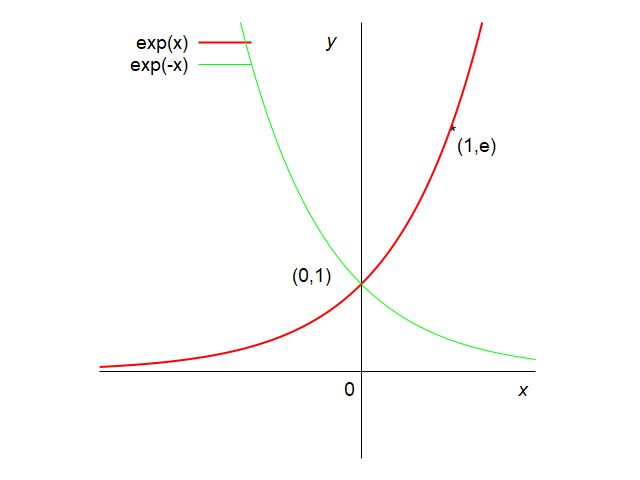
\includegraphics[width=\textwidth]{exp.png}
% 				\end{center}
% 		\end{columns}
% 		\end{minipage}
% \end{frame}

% \subsection{対数関数について}
% \begin{frame}
% 	\frametitle{対数関数}
% 		「指数と対数は表裏一体」で、逆関数の関係
% 		\vspace{-5mm}
% 		\begin{align*}
% 			\textcolor{blue}{a}^{\textcolor{red}{x}} = \textcolor{green}{M} \Leftrightarrow \textcolor{red}{x}= \log_{\textcolor{blue}{a}} \textcolor{green}{M}
% 		\end{align*}
% 		\centering
% 		\begin{minipage}{.95\textwidth}
% 			\begin{columns}[c, onlytextwidth]
% 				\column{.58\linewidth}
% 					\begin{block}{指数と対数}
% 						\begin{itemize}
% 							\item 指数：
% 							\textcolor{blue}{底}に\textcolor{red}{指数}を作用 $\rightarrow$ \textcolor{green}{真数}
% 								\vspace{-3mm}
% 								\begin{align*}
% 									f(x) = \textcolor{blue}{a}^{\textcolor{red}{x}}
% 								\end{align*}
% 							\item 対数：
% 							\textcolor{green}{真数}は\textcolor{blue}{底}にどんな\textcolor{red}{指数}を\\与えたもの？
% 							\vspace{-3mm}
% 								\begin{align*}
% 									f(x) = \log_{\textcolor{blue}{a}} \textcolor{green}{M}
% 								\end{align*}
% 						\end{itemize}
% 					\end{block}
% 				\column{.4\linewidth}
% 				% \begin{block}{グラフで見れば}
% 					% 底としてネイピア数を用いた場合、
% 					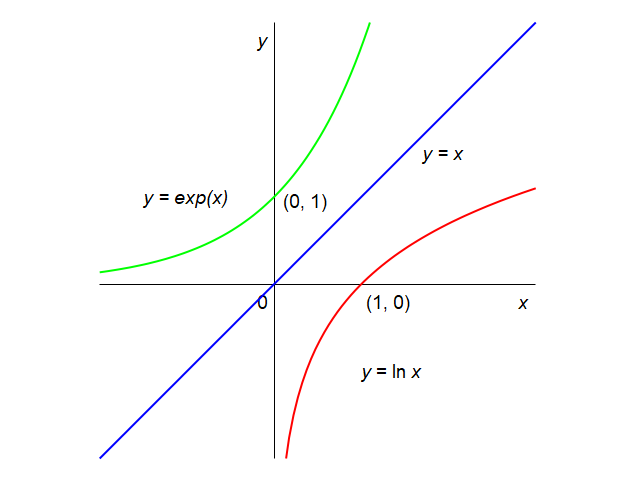
\includegraphics[width=\textwidth]{exp_ln.png}
% 					$y=x$に関して対称
% 				% \end{block}
% 			\end{columns}
% 		\end{minipage}
			
% \end{frame}

% \begin{frame}
% 	\frametitle{対数の性質}
% 		\begin{block}{対数の性質}
% 			\begin{itemize}
% 				\item 任意の正の実数 $M,N$ に対して
% 				\begin{itemize}
% 					\item 対数同士の足し算は真数の掛け算⇒ $\ln (M \times N) = \ln M + \ln N$
% 					\item 対数同士の引き算は真数の割り算⇒ $\ln(M \divisionsymbol  N) = \ln M - \ln N$
% 					\item 真数の冪は冪を掛け算に⇒ $\ln M^p = p \ln M$
% 					\item 真数の逆数はマイナスを付けて⇒ $\ln \dfrac{1}{M} = -\ln M$
% 					% \item $\ln 1 = 0$
% 				\end{itemize}
% 			\end{itemize}
% 		\end{block}

% 		\begin{block}{対数の使い方}
% 			\begin{itemize}
% 				\item 大きな数を桁数でざっくり見るときに便利
% 				\item \href{https://ja.wikipedia.org/wiki/対数スケール}{\alert{対数スケールのWikiへのリンク}}
% 			\end{itemize}
% 		\end{block}
% \end{frame}

% \begin{frame}
% 	\frametitle{対数グラフ}
% 	\begin{columns}[c, onlytextwidth]
% 		\column{.48\linewidth}
% 			\begin{block}{片対数グラフ}
% 				\begin{itemize}
% 					\item 指数関数で表される数式 \\$y=\exp(ax + b)$
% 					\item \alert{両辺の対数を取る}と\\$\ln y = ax + b$
% 				\end{itemize}

% 				\begin{itemize}
% 					\item 縦軸を対数目盛としたグラフで\\\alert{傾きが $a$、$y$ 切片が $b$の直線}
% 					\item 指数の異なる指数関数を\\片対数プロットすると右図
% 				\end{itemize}
% 			\end{block}
% 		\column{.48\linewidth}
% 			\centering
% 			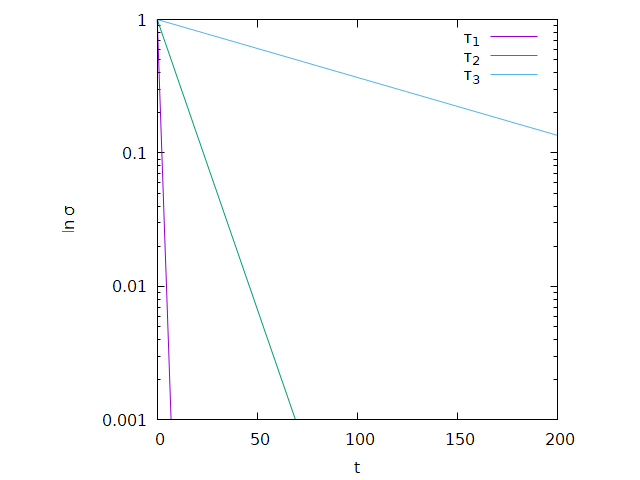
\includegraphics[width=\textwidth]{relux_6.png}
% 	\end{columns}
% \end{frame}

% \begin{frame}
% 	\frametitle{対数グラフ}
% 	\begin{columns}[T, onlytextwidth]
% 		\column{.52\linewidth}
% 			\begin{block}{両対数グラフ}
% 				\begin{itemize}
% 					\item 極端に範囲の広いデータを扱え\\ \alert{粘弾性スペクトルは通常この形}
% 					\item 冪関数 $y = x^a$ を線型で処理可能
% 					\begin{align*}
% 						\log y = a \log x
% 					\end{align*}
% 					\item 傾きがベキに対応
% 					\item 冪関数は両対数グラフで
% 				\end{itemize}
% 			\end{block}
% 		\column{.46\linewidth}
% 			\centering
% 			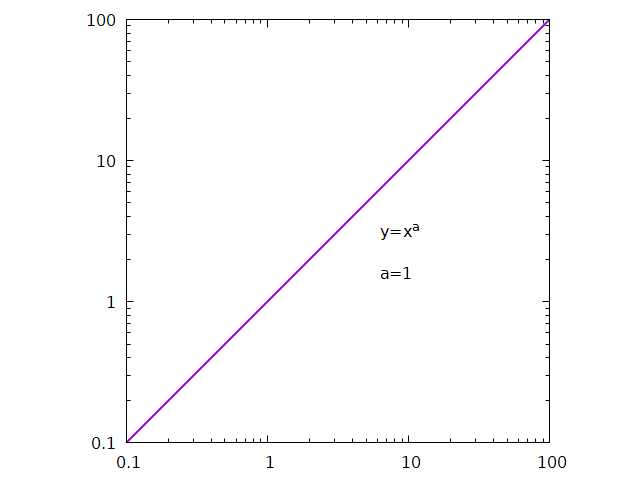
\includegraphics[width=\textwidth]{beki.png}

% 			% で\\プロットした例
% 	\end{columns}
	
% \end{frame}

\section{微積分について}
\subsection{微分について}
\begin{frame}
	\frametitle{微分の考え方}
		\centering
		\begin{minipage}{.9\textwidth}
			\begin{columns}[c, onlytextwidth]
			\column{.48\linewidth}
				\begin{block}{微分とは}
					\begin{itemize}
						\item 対象とする関数が
						\item \alert{注目する点の周り}で
						\item どう振る舞うか？
					\end{itemize}
				\end{block}
				\begin{alertblock}{ざっくりとは}
					\begin{itemize}
						\item 入力が増加したとき
						\begin{itemize}
							\item 微分が正 $\Leftrightarrow$ 出力は増加
							\item 微分が負 $\Leftrightarrow$ 出力が減る
						\end{itemize}
					\end{itemize}
				\end{alertblock}
			\column{.48\linewidth}
				\begin{block}{細かく言えば}
					\begin{itemize}
						\item 接線の「傾き」\\
						変数と関数の増分の\alert{「比」}
						\item \alert{変数の増分を無限小}
					\end{itemize}
					\centering
					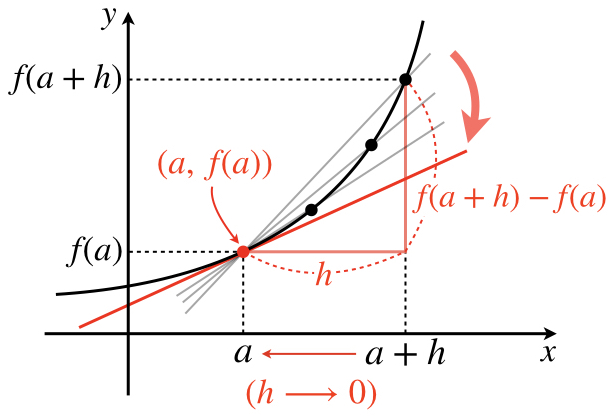
\includegraphics[width=.8\textwidth]{bibun.jpeg}
				\end{block}
		\end{columns}
		\end{minipage}
\end{frame}

\begin{frame}
	\frametitle{自転車のライトで微分をイメージ}
		\begin{columns}[T, onlytextwidth]
			\column{.7\linewidth}
				\begin{block}{自転車のライトは、}
					\begin{itemize}
						\item 速度を上げると明るく止まると消える。
						\begin{itemize}
							\item 明るさが瞬間的な速度
							\item 微分の値の大小に対応
						\end{itemize}
						\item \alert{明るさ $\Leftrightarrow$ 非常に短い時間あたりに進める距離}
					\end{itemize}
				\end{block}
			\column{.3\linewidth}
				\begin{center}
					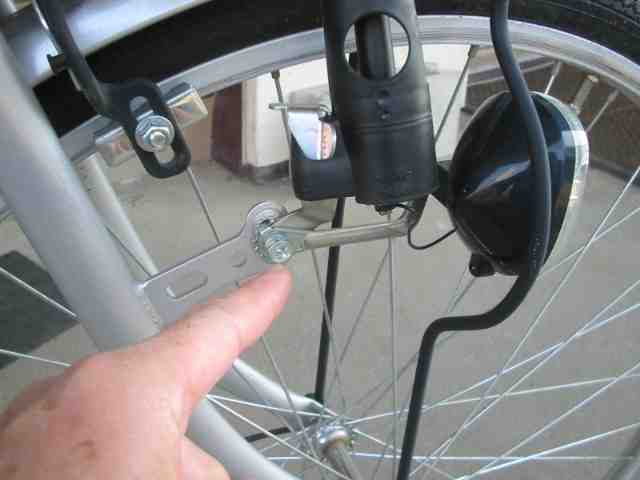
\includegraphics[width=\textwidth]{bike.jpg}
				\end{center}
		\end{columns}
		\begin{alertblock}<2>{微分の表すもの}
			\begin{itemize}
				\item 微分で見ることで、関数の瞬間的な振る舞いがわかる。
				\begin{itemize}
					\item 微分大 $\Leftrightarrow$ その瞬間に変化量が大きい
					\item 微分小 $\Leftrightarrow$ その瞬間にはあまり変化しない。
				\end{itemize}
			\end{itemize}
		\end{alertblock}
\end{frame}

\begin{frame}
	\frametitle{自転車のライトは微分と同じ}
	\begin{block}{距離と速度の関係}
		\begin{itemize}
			\item 時間 $t$ の関数として進んだ距離 $l$ を $l(t)$ と表したとき、
			\item \textcolor{red}{その微分を取れば各瞬間での速度 $v(t)$}となる。
		\end{itemize}
	\end{block}
		\begin{center}
			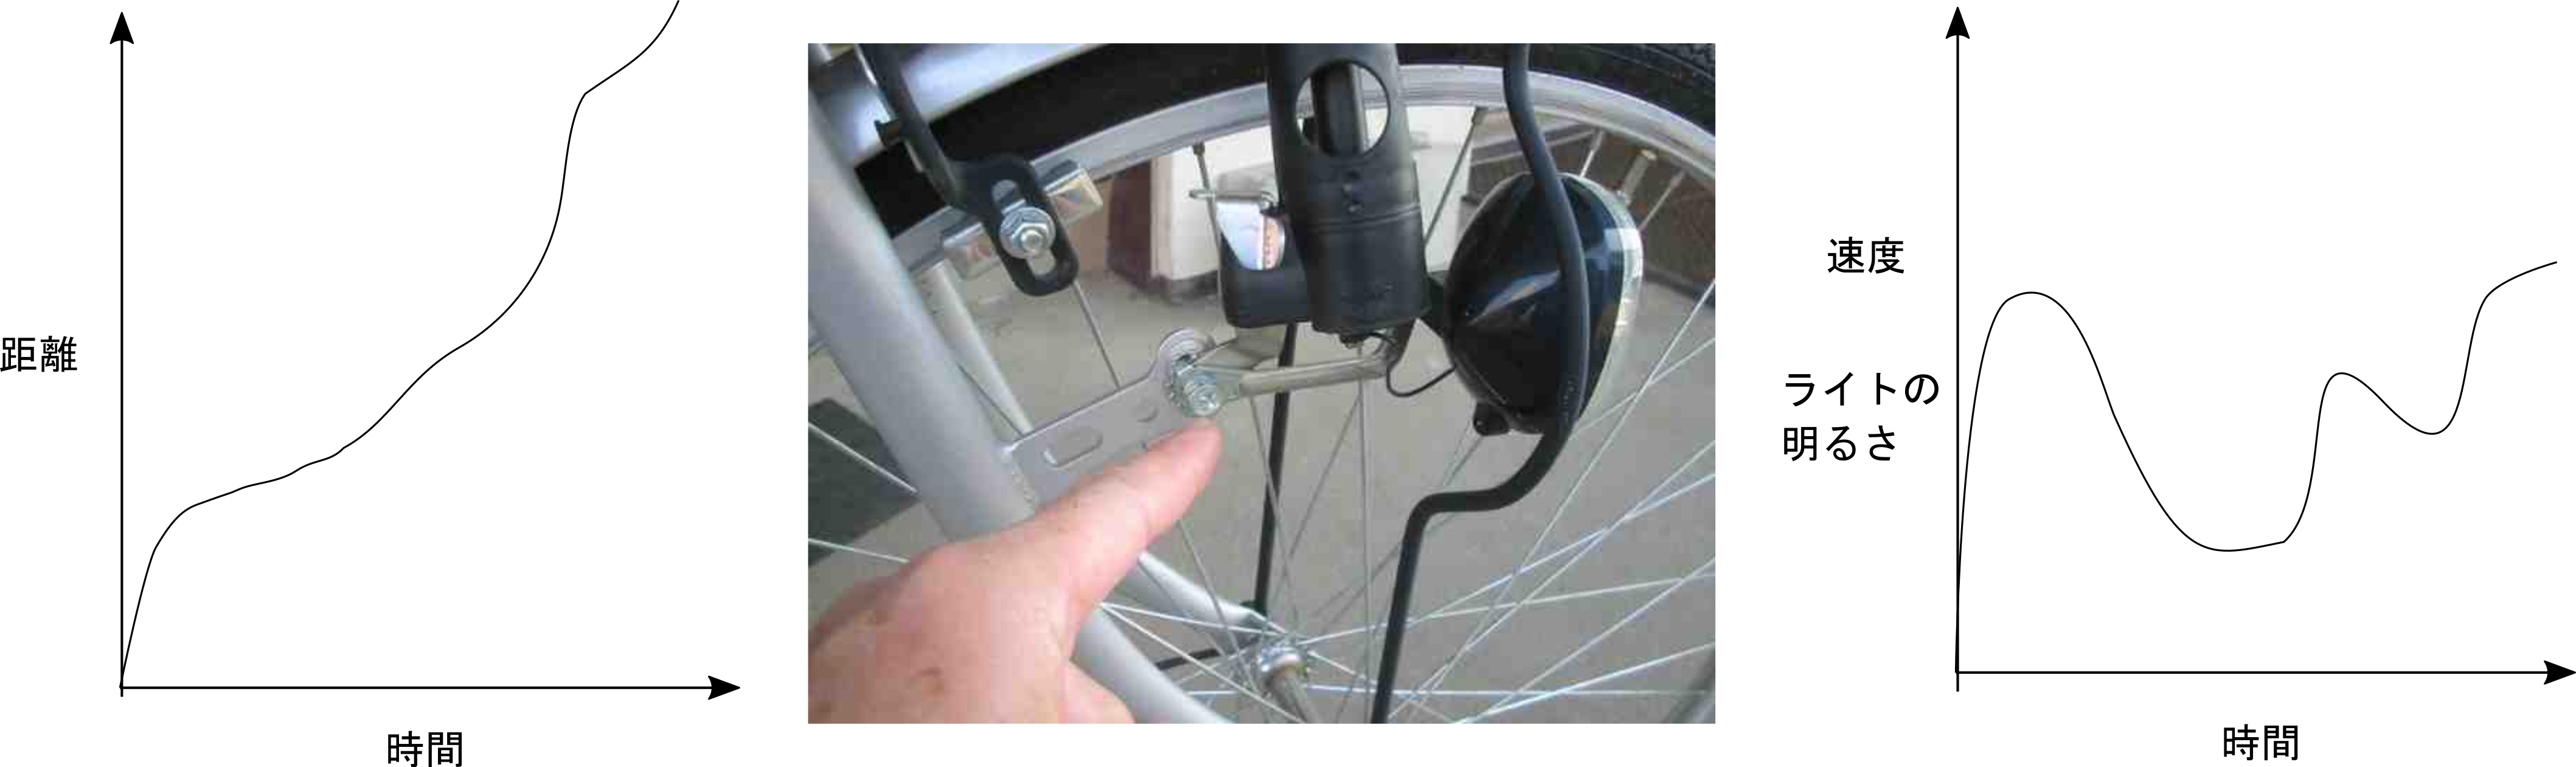
\includegraphics[width= .6\textwidth]{Move_light.png}
		\end{center}

		\vspace{-2mm}
	\begin{alertblock}{注意点}
		\begin{itemize}
			\item このアナロジーは微分値が正の場合のみ。⇔微分は負の値も
		\end{itemize}
	\end{alertblock}
\end{frame}

\begin{frame}
	\frametitle{最小限の微分の知識}
	% ここでの学習に必要となる最小限の微分関連の事項
	\begin{block}{微分の記法}
		\begin{itemize}
			\item $f(x)$ を $x$ で微分を、$\dv{f(x)}{x}$ と書き表す。
			\item \alert{d が微小量}を表し、（分母：変数）と（分子：関数）との\alert{僅かな変化の比}
		\end{itemize}
	\end{block}
	\vspace{-3mm}
	\footnotesize
	\renewcommand{\arraystretch}{2}
	\begin{table}[tb]
		\begin{center}
			\begin{tabular}{|c|c|c|} \hline
				微分の対象		& 公式							& メモ \\ \hline \hline
				冪の微分		& $\dd{}x^a = ax^{a-1}$ 		&  多項式では線形性も利用\\ \hline
				指数関数の微分	& $\dd{}\exp(x) = \exp(x)$ 		&  ネイピア数の場合\\ \hline
				自然対数の微分	& $\dd{}\ln x = \dfrac{1}{x}$ 	& 底がネイピア数 \\ \hline
			\end{tabular}
		\end{center}
	\end{table}
	\renewcommand{\arraystretch}{1.}
\end{frame}

\subsection{積分について}
\begin{frame}
	\frametitle{積分の2つのイメージ（定積分）}
	\centering
	\begin{minipage}{.9\textwidth}
		\begin{columns}[c, onlytextwidth]
		\column{.48\linewidth}
			\begin{block}{定積分は面積}
				\begin{itemize}
					\item 直感的には「面積」
					\begin{itemize}
						\item \textcolor{green}{微小な刻み $\dd x$} と
						\item \textcolor{red}{$f(x)$} との積（面積：\\グラフの台形）を
						\item \textcolor{blue}{積算}する。
						\vspace{-4mm}
						\small{
							\begin{equation*}
								\left[ F(x) \right]_a^b = \textcolor{blue}{\int_a^b} \textcolor{red}{f(x)} \textcolor{green}{\dd x}
							\end{equation*}
						}

					\end{itemize}
					\item 積分記号 $\int$ は、
					\begin{itemize}
						\item 和を表すSumから
						\item Sを縦方向に長く
					\end{itemize}
				\end{itemize}
			\end{block}
		\column{.5\linewidth}
			\centering
			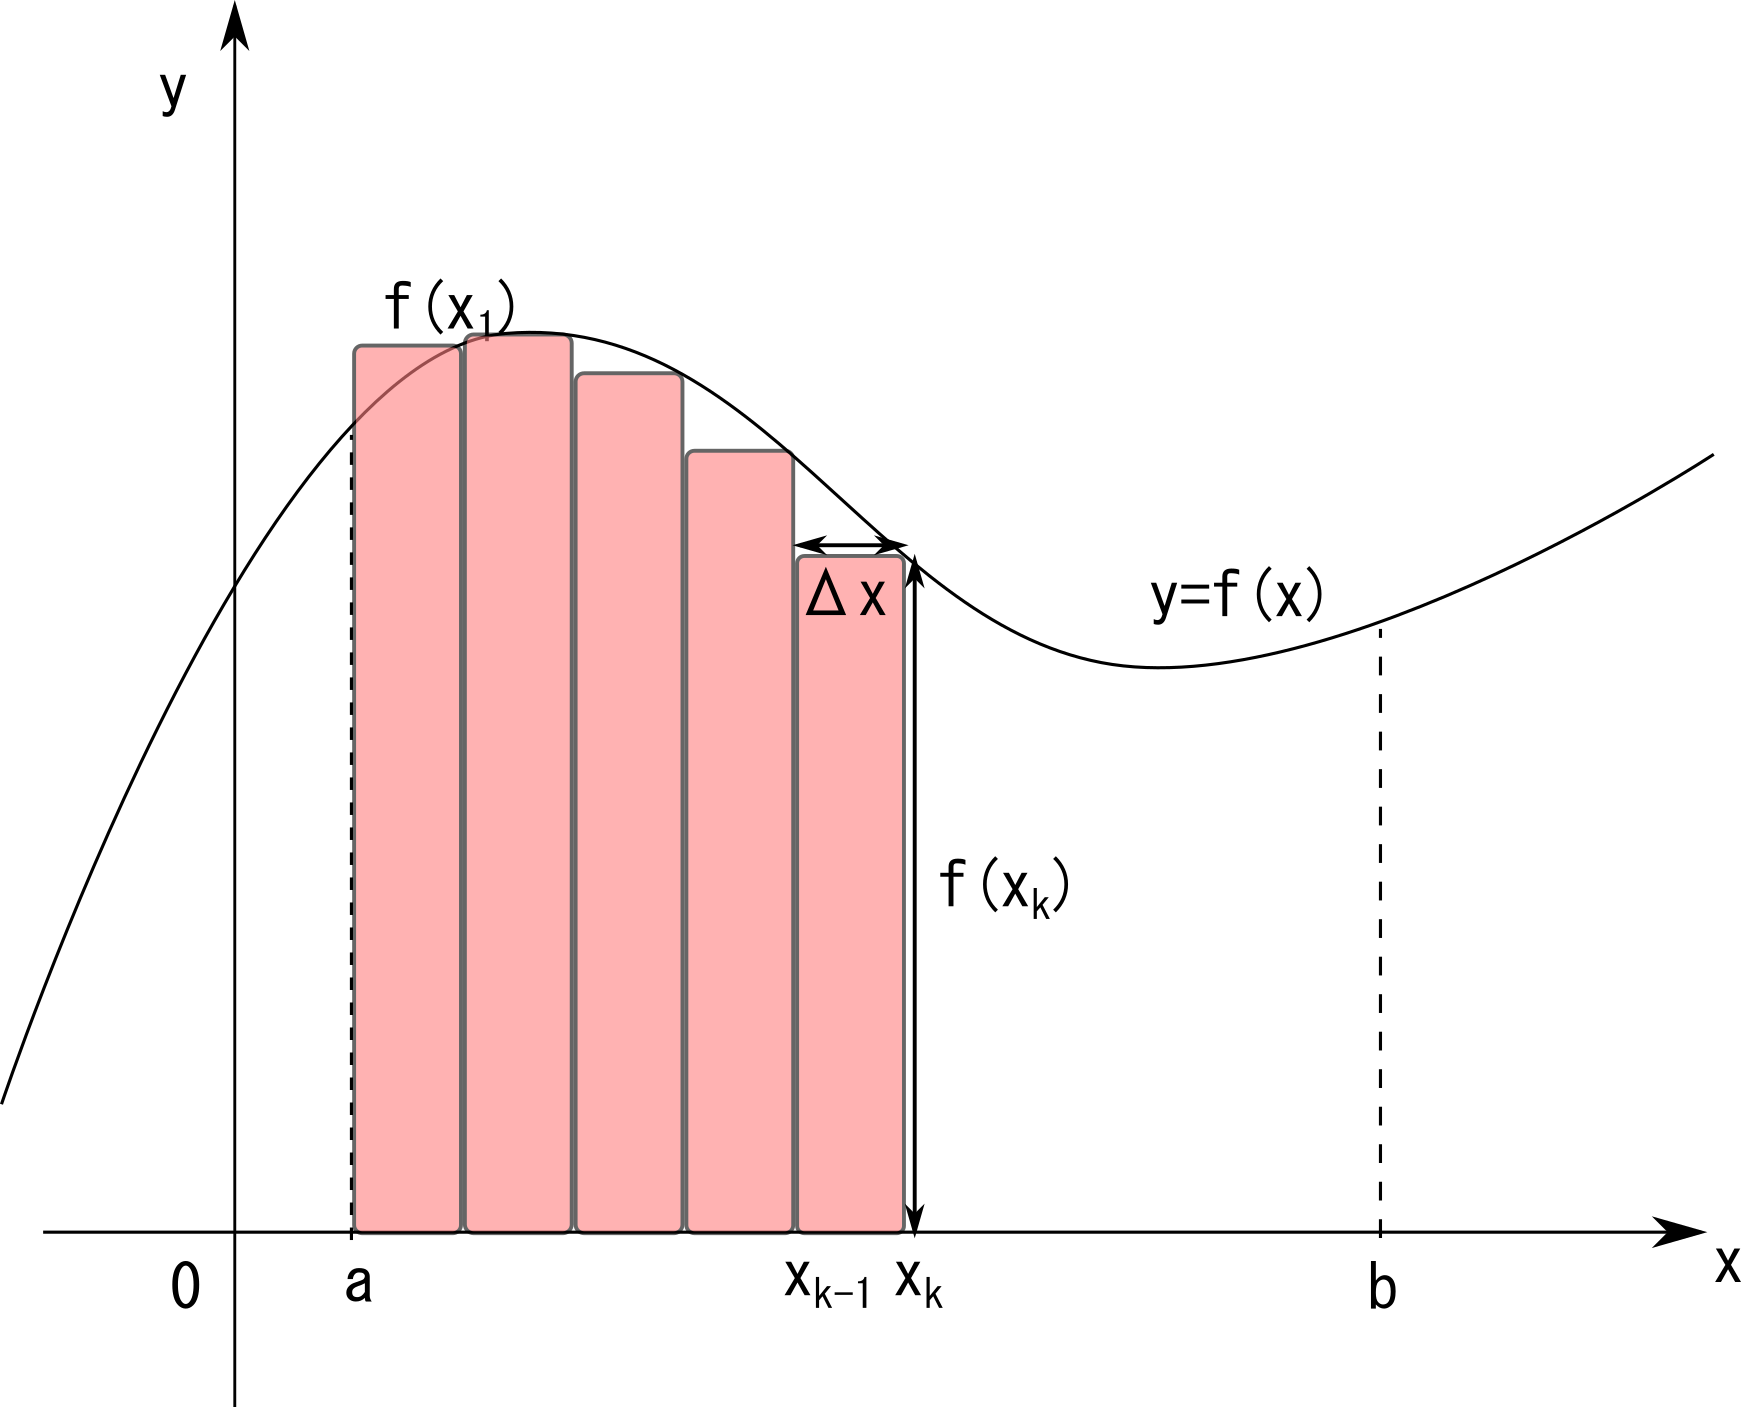
\includegraphics[width=.5\textwidth]{integral.png}
			\begin{alertblock}{自動車の速度の例}
				\begin{itemize}
					\item 速度が $v(t)$ のとき、
					\item 時刻 $t_0$ から $t_1$ までに\\進んだ距離 $L$ は、
				\end{itemize} 
				\vspace{-5mm}
				\small
				\begin{align*}
					L=\int_{t_0}^{t_1} v(t) \dd t
				\end{align*}
			\end{alertblock}		
	\end{columns}
	\end{minipage}
\end{frame}

\begin{frame}
	\frametitle{積分の2つのイメージ（微分の逆操作）}
		\begin{block}{微分の逆操作としての不定積分}
			\begin{itemize}
				\item 微分するとその関数 $f(x)$ に一致するような
				\item 原始関数 $F(x)$ を求める操作
				\begin{itemize}
					\item 積分範囲を定めない（不定）
					\item このとき、\alert{定数 $C$ （積分定数）だけ不定値}が出る。
				\end{itemize}
					\begin{align*}
						F(x) = \int f(x) \dd x +C
					\end{align*}
				\item \alert{（逆操作）}両辺を微分すれば、元の関数
					\begin{align*}
						\dv{x} F(x) = f(x)
					\end{align*}
			\end{itemize}
		\end{block}
\end{frame}

\subsection{微積分と微分方程式}
\begin{frame}
	\frametitle{微積分の直感的理解}
	\begin{block}{微積分を使えば、}
		\begin{itemize}
			\item 微分で瞬間の描像を取り出し、
			\item 積分で全体のふるまいを総量として把握。
		\end{itemize}
	\end{block}
	\vspace{3mm}
	\centering
	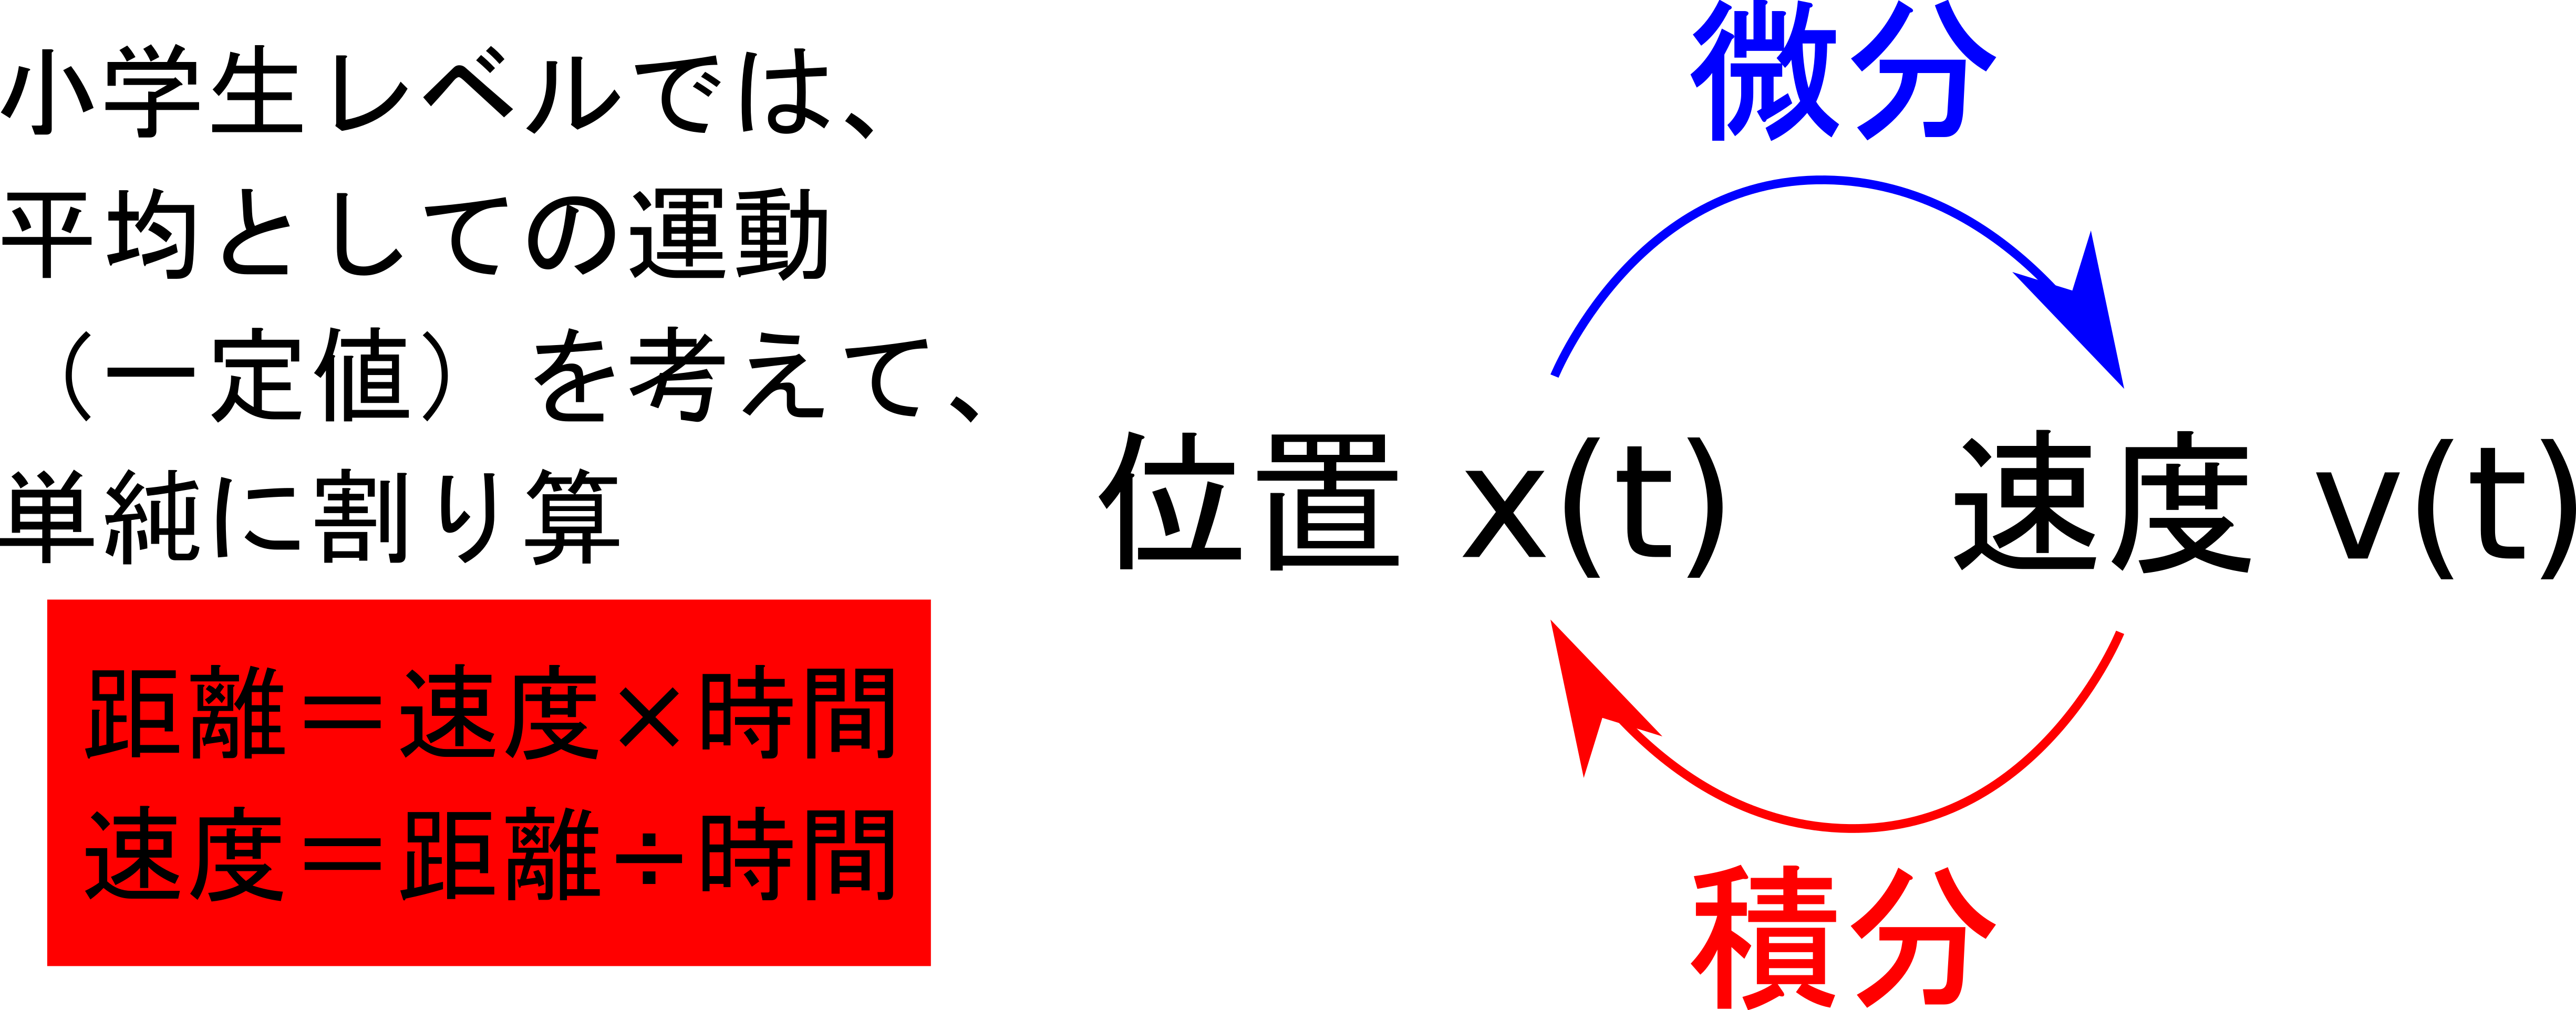
\includegraphics[width=.8\textwidth]{biseki.png}
\end{frame}

\begin{frame}
	\frametitle{微分で表される自然事象}
		\vspace{-2mm}
		\begin{alertblock}{微分方程式とは？}
			\begin{itemize}
				\item 物理現象や化学現象を\alert{「関数の微分の形で記述」}したもの
			\end{itemize}
		\end{alertblock}
			\begin{itemize}
				\item<2-> たとえば、「放射性物質の崩壊」等の、一次反応と呼ばれる化学現象を記述する頻出の微分方程式の形
			\vspace{-2mm}
				\small{\begin{align*}
					\textcolor{red}{\dv{t} N(t)} = \textcolor{blue}{-aN(t)}
				\end{align*}}
				\vspace{-6mm}
				\item<3-> この式の意味は
				\begin{itemize}
					\item 左辺は\textcolor{red}{時間の関数である $N(t)$ の時間変化を微分の形}
					\item 右辺は\textcolor{blue}{$N(t)$ の量に比例して減少（負号のため）}を表す
					% \item 定数 $a$ は [1/T] の次元を持つ
				\end{itemize}
			\end{itemize}
		
		\vspace{2mm}
		\centering
			\uncover<4>{\alert{\large{（ポイント）積分を使って、方程式を解く。}}}
\end{frame}

\begin{frame}
	\frametitle{微分方程式を解く (1)}
			\begin{itemize}
				\item 変数を両辺に振り分ける。
			\vspace{-3mm}
				% \small{
				\begin{align*}
					\dfrac{\dd N}{N} = -a\dd  t
				\end{align*}
				% }
			\vspace{-8mm}
				\item 両辺を積分する。
			\vspace{-3mm}
				% \small{
				\begin{align*}
					\int \dfrac{\dd N}{N} = -a \int \dd  t \\
					\ln N = -at + C
				\end{align*}
				% }
			\vspace{-8mm}
				\item 指数関数に書き直し
			\end{itemize}
			\vspace{-3mm}
				\begin{align*}
					N=\exp(-at + C) = \exp(C) \times \exp(-at) = C' \exp(-at)
				\end{align*}
\end{frame}

\begin{frame}
	\frametitle{微分方程式を解く (2)}
			\begin{itemize}
				\item 初期条件を考慮して変数を決める
				\begin{itemize}
					\item $t=0$での初期濃度が$N_0$とすると
					\vspace{-3mm}
					\begin{align*}
						N(t=0) &= C' \exp(-a*0) = N_0 \\
						\therefore\; C' = N_0
					\end{align*}

					\item $a$ は [1/T] の次元なので、時間の次元を持った $1/\tau$ と書き換え
					\vspace{-3mm}
					\begin{align*}
						a = \dfrac{1}{\tau}
					\end{align*}
				\end{itemize}
				\item 結局、
				% \small
				\begin{align*}
					N= N_0 \exp \left(-\dfrac{t}{\tau} \right)
				\end{align*}
			\end{itemize}
\end{frame}

\begin{frame}
	\frametitle{指数関数的減少の具体的な例}
		\begin{columns}[c, onlytextwidth]
			\column{.48\linewidth}
				\begin{block}{指数関数的減少とは？}
					\begin{itemize}
						\item 下式をグラフに表すと右図

					\vspace{-3mm}
						\small{\begin{align*}
							N(t) = N_0 \exp \left(-\dfrac{t}{\tau} \right)
						\end{align*}}
					\vspace{-5mm}
						\item 時間経過に伴い濃度が減少し $t = \tau$ において
					
					\vspace{-3mm}
						\small{\begin{align*}
							N(\tau) 
							&= N_0 \exp(-1)\\ 
							&= \dfrac{N_0}{e}
						\end{align*}}
						\end{itemize}
				\end{block}
			\column{.48\linewidth}
				\begin{center}
					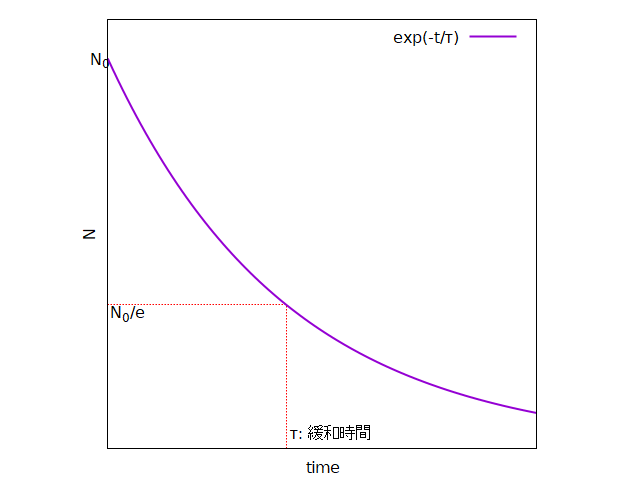
\includegraphics[width=.7\textwidth]{relux_1.png}
				\end{center}
				\vspace{-3mm}
				\begin{alertblock}{緩和時間とは、}
					\begin{itemize}
						\item 時間の次元を持つ $\tau$ は、
						\item 初期濃度の $\dfrac{1}{e}$ となる時間
					\end{itemize}
				\end{alertblock}
		\end{columns}
\end{frame}

\begin{frame}
	\frametitle{緩和時間の（一つの）考え方}
		\begin{columns}[T, onlytextwidth]
			\column{.5\linewidth}
				\begin{block}{初期の減少速度は？}
					\begin{itemize}
						\item 濃度の式を時間で微分\\して減少速度は、
					\end{itemize}
					\vspace{-3mm}
						\small{\begin{align*}
							\dv{N(t)}{t} = -\dfrac{N_0}{\tau} \exp \left(-\dfrac{t}{\tau} \right)
						\end{align*}}
					% \vspace{-5mm}
					\begin{itemize}
						\item $t=0$ での減少速度は
					\end{itemize}
					\vspace{-3mm}
						\small{\begin{align*}
							\dv{t}N(0) &=-\dfrac{N_0}{\tau} \exp \left(-\dfrac{0}{\tau} \right) \\
							&=-\dfrac{N_0}{\tau}
						\end{align*}}
				\end{block}
			\column{.46\linewidth}
				\begin{alertblock}{緩和時間の意味}
					初期速度を維持して減少\\すると、$t=\tau$ で濃度が 0
				\end{alertblock}
				\begin{center}
					\textcolor{red}{}
					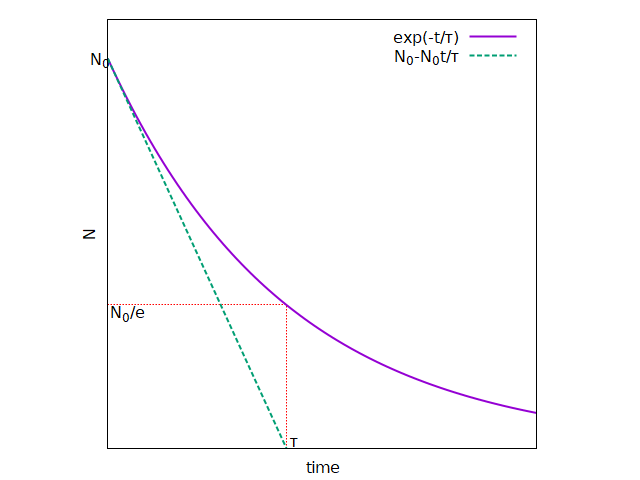
\includegraphics[width=\textwidth]{relux_2.png}
				\end{center}
		\end{columns}
\end{frame}

% \section{力と仕事を物理モデルで}

% \subsection{次元についてもう少し}
% \begin{frame}
% 	\frametitle{次元解析とは}
% 	\begin{block}{次元解析とは？}
% 		\begin{itemize}
% 			\item 物理量における各種の次元から、
% 			\item 複数の物理量の間の関係を予測すること
% 		\end{itemize}
% 	\end{block}
% 	\begin{block}{「次元一致の原理」}
% 		\begin{itemize}
% 			\item 物理的な関係を表す数式において、
% 			\item 両辺の次元が一致しなくてはならない。
% 			\item この規則を逆に利用すると、
% 			\begin{itemize}
% 				\item 既知の量を組み合わせて求めたい未知の物理量と、
% 				\item 次元に一致するように式を立てれば、
% 				\item それは正しい関係式になっている可能性が高い。
% 			\end{itemize} 
% 			% \item 例：バネの調和振動の周期 $T=A\sqrt{\dfrac{m}{k}}$
% 		\end{itemize}
% 	\end{block}
% \end{frame}

% \begin{frame}
% 	\frametitle{次元解析の例}
% 		バネの調和振動

% 		水平面上に質量 $m$ の物体をおき、垂直に立った壁と物体との間をばね定数 $k$ のばねで結ぶ。
% 		ばねの自然長の状態から物体を $x$ だけずらし、静かに手を離すと物体は振動運動を始める。
% 		このときの振動の周期（1振動にかかる時間）$T$ を与える式を推測する。
% 		水平面との摩擦や空気抵抗は考えない。

% 式に含まれるであろう定数は、物体の質量 m、ばね定数 k、初期変位 x の3つ
% 長さの次元を [L]、質量の次元を [M]、時間の次元を [T] とすれば、それぞれの定数および周期 T の次元は $[m]=[M],[k]={\mathsf{MT}}^{-2},[x]={\mathsf{L}},[T]={\mathsf{T}}$

% % {\displaystyle [m]={\mathsf {M}},[k]={\mathsf {MT}}^{-2},[x]={\mathsf {L}},[T]={\mathsf {T}}}である。
% % この中で長さの次元{\displaystyle {\mathsf {L}}}{\mathsf  {L}}を含んでいるのは初期変位 x のみなので、式に含めることができない。なぜなら式の左辺と右辺では次元が一致しなくてはならず、初期変位を含めるならば両辺に同じだけかける必要があり、それならば無くても同じだからである。

% % 次元が{\displaystyle {\mathsf {T}}}{\mathsf  {T}}になるように m と k を組み合わせる方法は一つしかない。結果次の式が求まる。

% % {\displaystyle T=A{\sqrt {\frac {m}{k}}}}T=A{\sqrt  {{\frac  {m}{k}}}}
% 比例係数 A は無次元量の定数で次元解析から求めることはできない。
% \end{frame}

% \begin{frame}
% 	\frametitle{無次元量について}
% 		\begin{block}{無次元量とは？}
% 			\begin{itemize}
% 				\item 無次元量は、無次元数、無名数とも呼ばれ、
% 				\item 全ての次元指数がゼロの量。
% 				\item 多くの無次元量が、1900年代初期、特に流体力学と熱伝導の分野で作られた。
% 			\end{itemize}
% 		\end{block}
% 		\begin{block}{その特徴}
% 			\begin{itemize}
% 				\item 無次元量の数値は\textcolor{red}{単位の選択に依らない。}
% 				\item 異なる系の\textcolor{red}{特徴を比較}するのにとても便利。
% 				\item 一般的な現象を特徴付ける物理量として、物理学、工学、経済など多くの分野で広く活用
% 				\item 当然、レオロジーでも。
% 			\end{itemize}
% 		\end{block}
% \end{frame}

% \begin{frame}
% 	\frametitle{無次元量の例}
% 		\begin{columns}[T, onlytextwidth]
% 			\column{.5\linewidth}
% 				\begin{block}{簡単な例として、比率}
% 					\begin{itemize}
% 						\item 同じ種類の2つの量の比として定義される
% 						% \begin{itemize}
% 						% 	\item 傾きは水平距離に対する鉛直距離の比
% 						% 	\item 「長さ」という同種の量の比
% 						% \end{itemize}
% 						\item 変形の尺度の「ひずみ」
% 						\begin{itemize}
% 							\item 変形前の長さに対する長さの変化の比
% 						\end{itemize}
% 						\item 濃度
% 						\begin{itemize}
% 							\item 例：アルコール度数はアルコール飲料の容積に対するエタノールの容積の比
% 						\end{itemize}
% 					\end{itemize}
% 				\end{block}
% 			\column{.46\linewidth}
% 				\begin{block}{もう少し難しい例}
% 					\begin{itemize}
% 						\item 偏差値\\母集団の中での位置
% 						\item レイノルズ数\\流れ場の状態を表す
% 						\item ヌセルト数\\伝熱を扱う
% 						\item プラントル数\\熱輸送と運動量輸送の比。
% 						% \item レイリー数\\熱対流を扱う
% 						\item ポアソン比\\ひずみ量の比。
% 					\end{itemize}
% 				\end{block}
% 		\end{columns}
% \end{frame}

% \begin{frame}
% 	\frametitle{無次元数の使い方}
% 	\begin{block}{レイノルズ数：}
% 		\begin{itemize}
% 			\item 流体の慣性力と粘性力（同じ次元の物理量）の比
% 			\item 流れ場の状態（運動量輸送における移流と拡散の比）を表す
% 		\end{itemize}
% 	\end{block}
% 	\begin{block}{その使い方}
% 		\begin{itemize}
% 			\item 形は同じで大きさが異なる物体回りの流れを比較
% 			\begin{itemize}
% 				\item 両者のレイノルズ数が同じであれば、
% 				\item 物体回りの流体の流れは相似となり
% 				\item サイズは異なるが本質的には同じ現象
% 			\end{itemize}
% 			\item 風洞実験でモデルと実機を比較
% 			\item  特に乱流を扱う際は必須のパラメーター
% 		\end{itemize}
% 	\end{block}
% \end{frame}

% \subsection{力、仕事、エネルギー}
% \begin{frame}
% 	\frametitle{力とは}
% 	\begin{block}{力とは}
% 		\begin{itemize}
% 			\item 「物体の状態を変化させる原因となる作用、\\
% 			その作用の大きさを表す物理量」
% 			\item \textcolor{red}{単純化した仮想的な状態（高校の物理）}として、\\
% 			「慣性系」で「保存力」を考える。 
% 			\begin{itemize}
% 				\item 力の定義は、結構面倒。
% 				\item「慣性系とか保存力って何？」の話はしない
% 				\item 現時点では\textcolor{red}{摩擦や熱を考えていない。}
% 			\end{itemize}
% 		\end{itemize}
% 	\end{block}
% 	% \begin{alertblock}{$F=ma$ の意味}
% 	% 	\begin{itemize}
% 	% 		\item $m$ という「質量（変化の受け難さ）」を持った物体に、
% 	% 		\item $F$ という「力」を作用すると、
% 	% 		\item $a$ という「加速度」で運動（状態変化）する。
% 	% 	\end{itemize}
% 	% \end{alertblock}
% \end{frame}

% \begin{frame}
% 	\frametitle{仕事とエネルギー}
% 	\begin{columns}[c, onlytextwidth]
% 		\column{.48\linewidth}
% 			\begin{block}{仕事とは}
% 				\begin{itemize}
% 					\item 質点に力を作用し移動すること
% 					\item 仕事は作用させた力 $F$ と\\移動した距離 $s$ の積
% 				\end{itemize}
% 				\begin{center}
% 					
\includegraphics[width=.8\textwidth]{work.png}
% 				\end{center}
% 			\end{block}
% 		\column{.48\linewidth}
% 			\begin{block}<2->{エネルギーとは}
% 				\begin{itemize}
% 					\item 仕事をする能力のこと
% 					\item 物体や空間は状態変化に伴い\\エネルギーを蓄える
% 					\item 仕事とエネルギーの次元は同一
% 				\end{itemize}
% 			\end{block}
% 	\end{columns}
% 	\begin{block}<3>{仕事の次元と単位}
% 		\begin{itemize}
% 			\item 次元：[仕事] = [力][距離] = [$ML^2T^{-2}$]、単位：ジュール J
% 		\end{itemize}
% 	\end{block}
% \end{frame}

% \subsection{ポテンシャルと力と微積分}
% \begin{frame}
% 	\frametitle{仕事とポテンシャル}
% 		\begin{columns}[c, onlytextwidth]
% 			\column{.6\linewidth}
% 				\begin{block}{ポテンシャルとは}
% 			\begin{itemize}
% 				\item \alert{基準の状態}を定めて
% 				\begin{itemize}
% 					\item その着目する状態にするために
% 					\item 物体あるいは空間に加えた\alert{仕事の量}
% 				\end{itemize}
% 				\item 逆に言えば
% 				\begin{itemize}
% 					\item ある状態から基準の状態に戻るまでに
% 					\item \alert{外に取り出せるエネルギーの量}
% 				\end{itemize}
% 				\item 力が「\textcolor{red}{保存力}」の場合は
% 				\item ポテンシャルが「位置のみの関数の\\\textcolor{red}{状態量}」となる
% 			\end{itemize}
% 		\end{block}
% 			\column{.38\linewidth}
% 				\begin{block}{保存力の定義：}
% 					\begin{itemize}
% 						\item 仕事が経路によらない
% 					\end{itemize}
% 				\end{block}

% 				\begin{block}{状態量：}
% 					\begin{itemize}
% 						\item 系の状態だけで、\\一意に決まる物理量
% 					\end{itemize}
% 				\end{block}
% 		\end{columns}
% \end{frame}

% \begin{frame}
% 	\frametitle{ポテンシャルと力}
% 	\centering
% 	\begin{minipage}{.9\textwidth}
% 		\begin{columns}[c, onlytextwidth]
% 		\column{.6\linewidth}
% 			\only<1>{\begin{block}{ポテンシャル $U(\vb{r})$は}
% 				\begin{itemize}
% 					\item 基準の位置 $\vb{r_0}$ から
% 					\item 位置 $\vb{r}$ までの
% 					\item 力 $F(\vb{r})$ の積分であり、
% 					\item 位置ベクトル$\vb{r}$の関数
% 				\end{itemize}

% 				\vspace{-8mm}
% 				\begin{align*}
% 					W(\vb{r}) = \int_{\vb{r_0}}^{\vb{r}} F(\vb{r}) \dd \vb{r} = -U(\vb{r})
% 				\end{align*}
% 			\end{block}}
			
% 			\only<2>{\begin{block}{力 $F(\vb{r})$は}
% 				\begin{itemize}
% 					\item 任意の位置$\vb{r}$において
% 					\item ポテンシャル$U(\vb{r})$ を
% 					\item $\vb{r}$で微分すれば
% 				\end{itemize}
% 					\begin{align*}
% 						\dv{\vb{r}} U(\vb{r}) = -F(\vb{r})
% 					\end{align*}
% 			\end{block}}
			
% 			\only<3>{
% 				\begin{alertblock}{バネの場合は}
% 				\begin{itemize}
% 					\item 力は $F(x)=-kx$
% 					\item ポテンシャル $U(x)$ は
% 					\begin{align*}
% 						U(x) 
% 						&= -\int_0^x F(x') \dd x' \\
% 						&= \dfrac{1}{2}kx^2
% 					\end{align*}
% 				\end{itemize}
% 			\end{alertblock}
% 			}
% 		\column{.4\linewidth}
% 			\begin{center}
% 				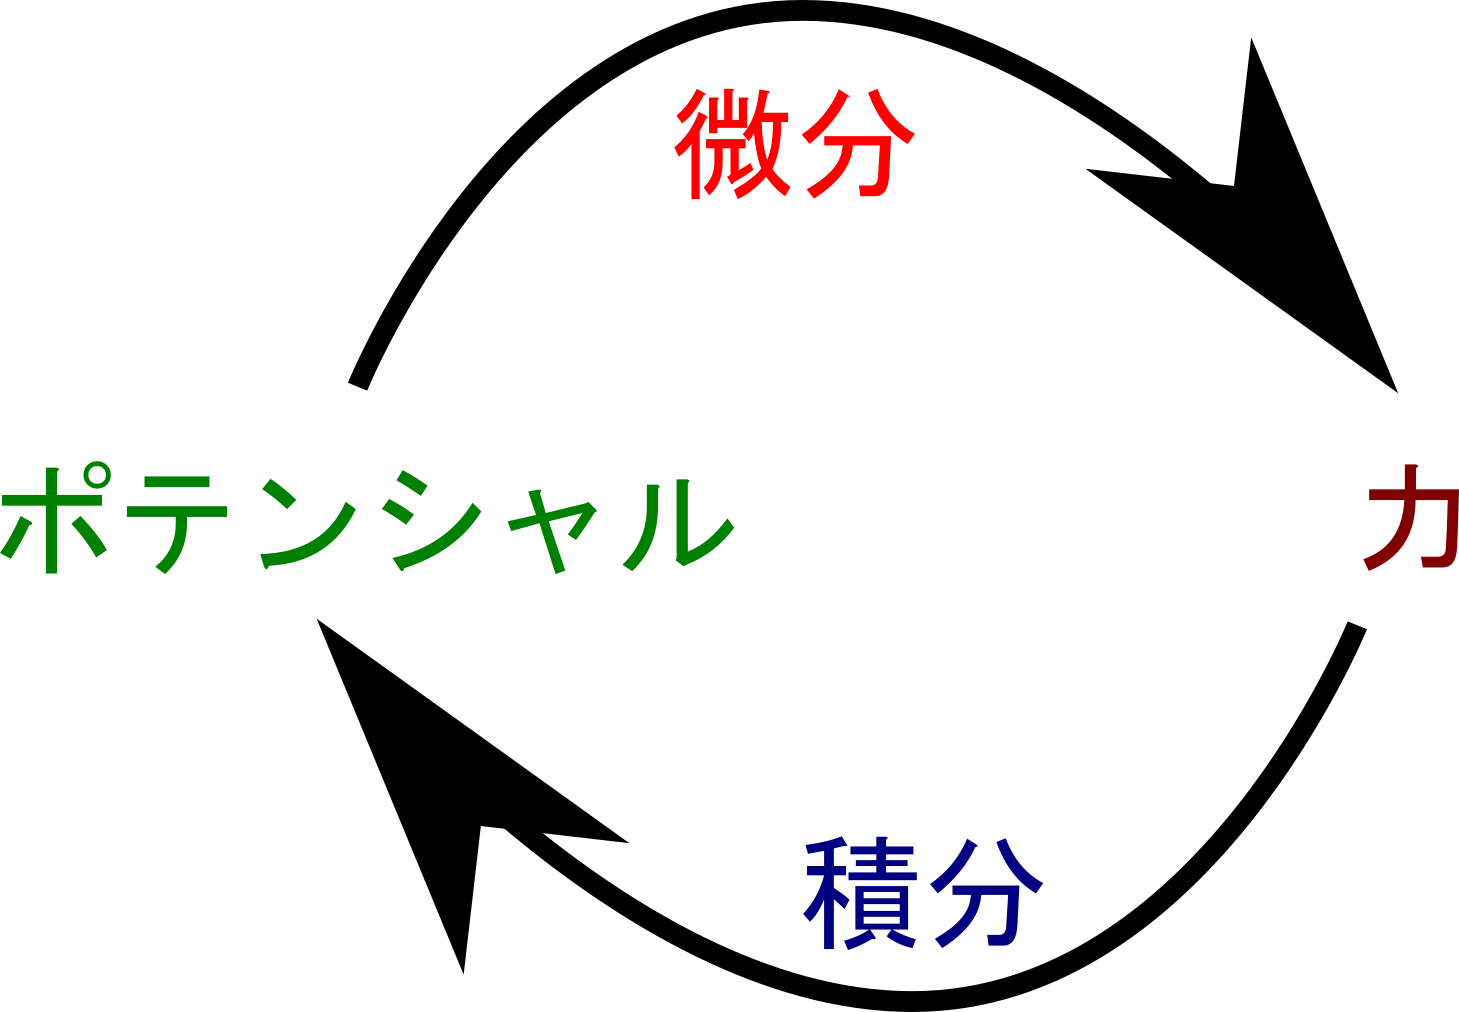
\includegraphics[width=\textwidth]{potential_power.png}

% 				ポテンシャルと力は\\互いに入れ子
% 			\end{center}
% 	\end{columns}
% 	\end{minipage}
	
% \end{frame}

% \subsection{摩擦と熱}
% \begin{frame}
% 	\frametitle{摩擦について}
% 		\begin{columns}[c, onlytextwidth]
% 			\column{.5\linewidth}
% 				\begin{block}{摩擦と熱とエネルギー}
% 					\begin{itemize}
% 						\item 摩擦力は非保存力
% 							\begin{itemize}
% 								\item ポテンシャルは状態量ではなく\\経路に依存
% 							\end{itemize}
% 						\item<2-> 内部の粒子の摩擦により、
% 							\begin{itemize}
% 								\item 粒子の運動エネルギーが増加し\\系全体の温度が上昇
% 								\item 非断熱系では、熱エネルギー\\として外界に散逸。
% 							\end{itemize}
% 						\item<3> \alert{非保存力も含めれば、\\系全体のエネルギーは保存}
% 					\end{itemize}
% 				\end{block}
% 			\column{.45\linewidth}
% 				\begin{center}
% 					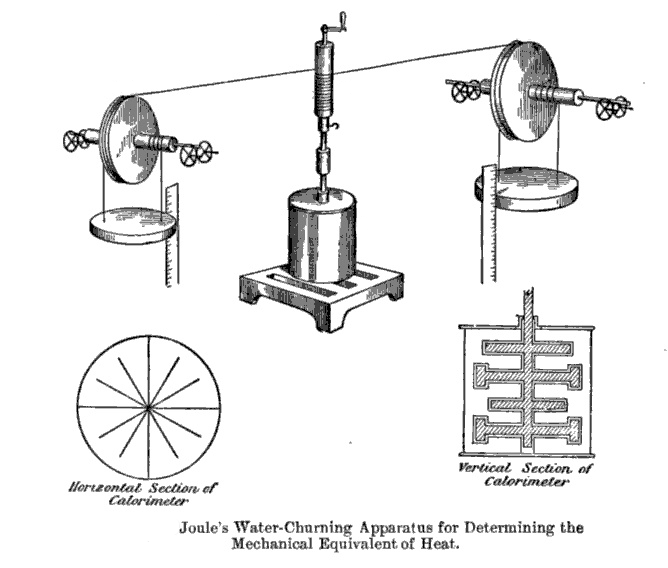
\includegraphics[width=\textwidth]{thermal_eng.png}
% 					ジュールの試験
% 				\end{center}
% 		\end{columns}
% \end{frame}


% % \section{この章のまとめ}
% \begin{frame}
% 	\frametitle{まとめ}
% 	% この章では、以下に示したような、ちょっとだけ小難しくなった数学と物理の事項を学びました。
% 		\begin{boxnote}
% 			\begin{itemize}
% 				\item 数学的な事項について
% 					\begin{itemize}
% 						\item 指数関数とその逆関数である対数関数の確認
% 						\item 微分が「瞬間的な振る舞い」、積分が「全体の量を把握」
% 						\item 簡単な微分方程式から「指数関数的な応答」を理解
% 					\end{itemize}
% 				\item 物理に関する事項として
% 					\begin{itemize}
% 						% \item 「次元解析」や「無次元量」について
% 						\item 力、仕事、エネルギー、ポテンシャルを確認し
% 						\item それら相互の関係と微積分について
% 						\item 摩擦と熱についても
% 					\end{itemize}
% 			\end{itemize}
% 		\end{boxnote}
% \end{frame}

% \appendix
% \backupbegin

% \section{数学関連のメモ}
% \subsection{指数の性質について}
% \begin{frame}
% 	\frametitle{指数の性質（整数への拡張）}
% 	\begin{columns}[T, onlytextwidth]
% 		\column{.5\linewidth}
% 			\begin{block}{指数が 0 の場合は？: $a^0$}
% 				\vspace{-5mm}
% 				\begin{align*}
% 				&a^n \times a^0 =a^{(n+0)} = a^n \\
% 				\therefore \;\;&a^0 = 1
% 				\end{align*}
% 			\end{block}
% 			\begin{block}{負数への拡張: \\$a^{-k}$ ($k$ が正の整数)}
% 				\vspace{-5mm}
% 				\begin{align*}
% 					&a^k \times a^{-k} = a^{k+(-k)}=a^0=1 \\
% 					&\; \text{$a^k (\ne 0)$ で両辺を除すと、} \\
% 					&\therefore \; a^{-k} = \dfrac{1}{a^k}
% 				\end{align*}
% 				指数が負 $\Rightarrow$ 指数が正の逆数
% 			\end{block}
% 		\column{.46\linewidth}
% 		\begin{alertblock}{指数同士の割り算}
% 			\begin{itemize}
% 				\item \textcolor{red}{割り算は指数が負}に\\なると考える。
% 				\item 結局、以下のように\\\textcolor{red}{指数の引き算}となる。
% 			\end{itemize}
% 			\begin{align*}
% 				a^n \textcolor{red}{\divisionsymbol  a^m} 
% 					&=a^n \textcolor{red}{\times \dfrac{1}{a^m}} \\
% 					&= a^n \textcolor{red}{\times a^{-m}} \\
% 					&= a^{n + (-m)}
% 			\end{align*}
% 		\end{alertblock}
% 	\end{columns}	
% \end{frame}

% \begin{frame}
% 	\frametitle{指数の性質（有理数への拡張）}
% 		\begin{block}{}
% 			\begin{columns}[T, onlytextwidth]
% 				\column{.48\linewidth}
% 					\begin{itemize}
% 						\item $a^{\frac{1}{n}}$（$n$ は整数）を $n$ 乗\\することを考える。
% 							\begin{equation*}
% 								(a^{\frac{1}{n}})^n=a^{\frac{1}{n} \times n} = a
% 							\end{equation*}
% 						\item すなわち、\\ $a^{\frac{1}{n}}$ の $n$ 乗が $a$
% 					\end{itemize}
% 				\column{.48\linewidth}
% 					\begin{itemize}
% 						% \item 実数 $x$ に対して、
% 						\item $x$ を $n$ 乗（$n$ は正の整数）すると $y$ になるとき、
% 						\begin{itemize}
% 							\item $y$ を「$x$ の $n$ 乗根」
% 							\item $\sqrt[n]{x}$ と表記
% 						\end{itemize}
% 					\end{itemize}
% 			\end{columns}
% 		\end{block}
% 	\begin{alertblock}{指数が分数の場合}
% 		\begin{itemize}
% 			\item 分数の分母となる値を用いて累乗根を表し、
% 			\item 分子はそのべき乗を表すこととなり、
% 			\item 以下のように記述できる。
% 		\end{itemize}
% 		\begin{equation*}
% 		a^{\frac{m}{n}}=\sqrt[n]{a^m}
% 		\end{equation*}
% 	\end{alertblock}
% \end{frame}

% \section{演習問題 1}
% \subsection{「レオロジーで扱う関数について」}
% \begin{frame}
% 	\frametitle{「レオロジーで扱う関数について」}
% 	\small
% 		\begin{itemize}
% 			\item \textcolor<2>{black}{冪}とは、「\fbox{\textcolor<1>{white}{底}}」と呼ばれる正の数の右肩に「\fbox{\textcolor<1>{white}{指数}}」と呼ばれる数を載せた数式表現。
% 			\item 同じ底の累乗同士の掛け算は、\fbox{\textcolor<1>{white}{指数同士の足し算}}となる。
% 			\item 累乗のさらなる累乗は、\fbox{\textcolor<1>{white}{指数同士の掛け算}}となる。
% 			\item 指数同士の割り算は、\fbox{\textcolor<1>{white}{指数の引き算}}となる。
% 			\item 指数が分数の場合、分数の分母となる値が\fbox{\textcolor<1>{white}{累乗根}}を表し、分子はその\fbox{\textcolor<1>{white}{べき乗}}を表す。
% 			\item 物理的な議論では、底に\fbox{\textcolor<1>{white}{ネイピア数}} e を多用。
% 		\end{itemize}
% \end{frame}

% \backupend

\end{document}